\clearpage

\newenvironment{subs}
  {\begin{adjustwidth}{1em}{0pt}
  \nointerlineskip\leavevmode}
  {\end{adjustwidth}}


\section{Bit Error Rate}
\label{sec:bit_error_rate}
\begin{refsection}

\begin{tcolorbox}	
\begin{tabular}{p{2.75cm} p{0.2cm} p{10.5cm}} 	
\textbf{Header File}    &:& bit\_error\_rate\_*.h \\
\textbf{Source File}    &:& bit\_error\_rate\_*.cpp \\
\textbf{Version}        &:& 20171810 (Daniel Pereira)\\
                        &:& 20181424 (Mariana Ramos) \\
                        &:& 20180815 (Manuel Neves)\\
\end{tabular}
\end{tcolorbox}
Bit Error Rate is a rather intuitive concept and this block, at its simplest usage, does exactly what you'd expect it to: given two signals it compares them and outputs a binary vector indicating, for each bit, whether there was or not an error.\\
Additionally, this block does statistical analysis on the BER and outputs a file where the result of this analysis can be assessed.
The statistical analysis consists on the upper and lower bounds of the BER value, as well as its average value.\\
The block also allows having breakpoints on the BER analysis, outputting mid-reports (instead of only one final report).

\subsection*{Signals}
\begin{subs}
\subsubsection*{Input Signals}
\end{subs}
\hspace*{0.5in}\textbf{Number}: 2\\
\hspace*{0.5in}\textbf{Type}: Binary
\\
These two input signals are (interchangeably) the received binary sequence, from the MQAM Receiver output, and the transmitted signal, directly from the Binary Source.
\begin{subs}
\subsubsection*{Output Signals}
\end{subs}
\hspace*{0.5in}\textbf{Number}: 1\\
\hspace*{0.5in}\textbf{Type}: Binary
\\
The output signal is a binary vector of '1's and '0's, with the same length as the input signals, in which a '0' indicates the occurrence of an error and a '1' a successfully transmitted bit.


\subsection*{Input Parameters}

\begin{table}[H]
\centering
\begin{tabular}{|p{1.5cm}|p{1.5cm}|p{1.5cm}|p{7cm}|}
\hline
\textbf{Name}   & \textbf{Type} & \textbf{Default Value}    & \textbf{Description} \\ \hline
alpha           & double        & 0.05                      & Alpha is related with the confidence level required for the Upper and Lower bounds. \\ \hline
m               & integer       & 0                         & Defines how many bits are analysed in between mid-reports. When null there aren't any mid-reports. \\ \hline
lMinorant       & double        & $1\times10^{-10}$         & Defines the minimum value of the lower bound for the BER.\\ \hline
\end{tabular}
\end{table}


\subsection*{Block Constructor}

\begin{itemize}
  \item \textbf{BitErrorRate}(vector<Signal *> InputSig, vector<Signal *> OutputSig) :Block(InputSig,OutputSig)\{\};
\end{itemize}
This block's constructor expects, as any \textit{Block} object, an input of two vectors of Signal pointers, \textit{InputSig} and \textit{OutputSig}, containing the input/output signals described above.

\subsection*{Methods}

\begin{itemize}
  \item void \textbf{initialize}(void);
  \begin{itemize}
    \item[--] Sets symbol and sampling period and the \textit{firstValueToBeSaved} of the output signal, based on the input signals.
  \end{itemize}
  \item bool \textbf{runBlock}(void);
  \begin{itemize}
    \item[--] Computes output statistics and writes to BER.txt and mid-report\#.txt the obtained results.
  \end{itemize}
  \item double const \textbf{getConfidence}(double P);
  \begin{itemize}
    \item[--] Returns the value of the confidence level based on the private parameter \textit{alpha}.
  \end{itemize}
  \item void \textbf{setConfidence}(double P);
  \begin{itemize}
    \item[--] Defines the value of the \textit{alpha} parameter, based on the wished confidence.
  \end{itemize}
  \item int const \textbf{getMidReportSize}(int M);
  \begin{itemize}
    \item[--] Returns the value of the private parameter \textit{m}.
  \end{itemize}
  \item void \textbf{setMidReportSize}(int M);
  \begin{itemize}
    \item[--] Alters the value of the \textit{m} parameter, from its default.
  \end{itemize}
  \item double \textbf{getLowestMinorant}(double lMinorant);
  \begin{itemize}
    \item[--] Returns the value of the private parameter \textit{lMinorant}.
  \end{itemize}
  \item void \textbf{setLowestMinorant}(double lMinorant);
  \begin{itemize}
    \item[--] Alters the value of the \textit{lMinorant} parameter, from its default.
  \end{itemize}
\end{itemize}


\subsection*{Examples}
\begin{itemize}
    \item[--] One interesting test we can do with this block, is analyse how a certain parameter of the system affects de BER.
        In the following graph we demonstrate an example of how the Noise Spectral Density of the TI Amplifier on the receiver affects the BER:

        \begin{center}
        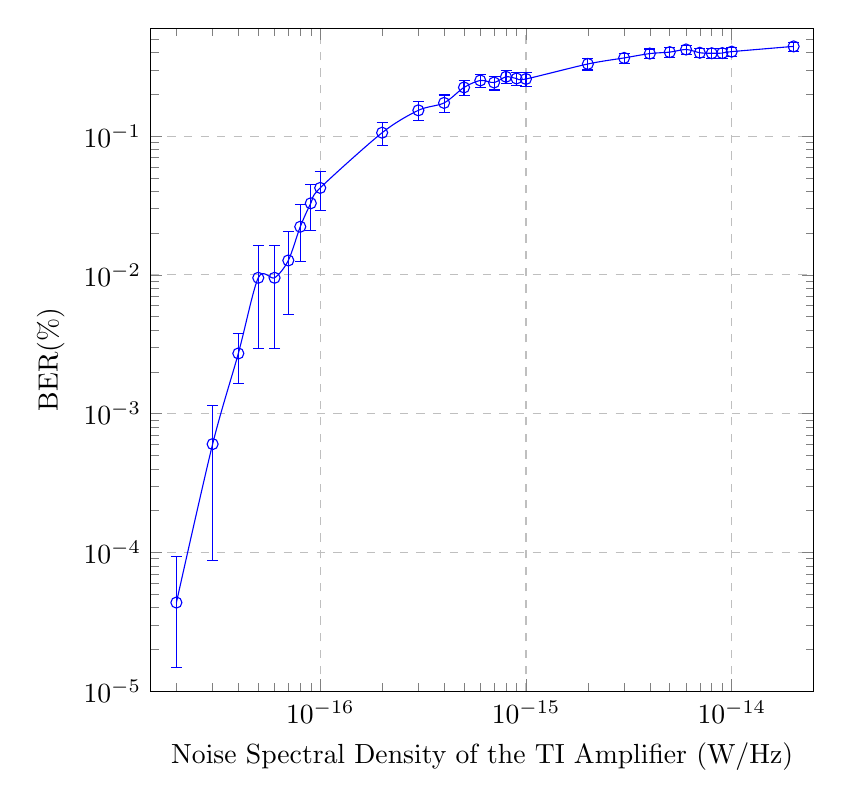
\begin{tikzpicture}
            \begin{axis}[
                height=10cm,
                width=10cm,
                xlabel=Noise Spectral Density of the TI Amplifier (W/Hz),
                ylabel=BER(\%),
                ymin=1e-5, ymax=0.6,
                xmin=1.5e-17, xmax=2.5e-14,
                ymode=log,
                xmode=log,
                ymajorgrids=true,
                xmajorgrids=true,
                grid style=dashed,
            ]
            \addplot[
                samples y=0,
                smooth,
                mark=o,
                blue,
                error bars/.cd, y dir=both, y explicit,
            ] plot coordinates {
                (2e-17,4.34783e-05) +=(0,4.9852e-05) -=(0,2.86804e-05)
                (3e-17,0.000603379) +=(0,0.000549511) -=(0,0.0005163459)
                (4e-17,0.00271521) +=(0,0.00108902) -=(0,0.00105709)
                (5e-17,0.0095339) +=(0,0.0068759) -=(0,0.00658128)
                (6e-17,0.0095339) +=(0,0.0068759) -=(0,0.00658128)
                (7e-17,0.0127119) +=(0,0.0078136) -=(0,0.00753854)
                (8e-17,0.0222458) +=(0,0.010046) -=(0,0.0098294)
                (9e-17,0.032839) +=(0,0.0119741) -=(0,0.0118224)
                (1e-16,0.0423729) +=(0,0.0134263) -=(0,0.0133331)
                (2e-16,0.105932) +=(0,0.020013) -=(0,0.0203095)
                (3e-16,0.153602) +=(0,0.023236) -=(0,0.023825)
                (4e-16,0.173729) +=(0,0.024342) -=(0,0.025055)
                (5e-16,0.224576) +=(0,0.026638) -=(0,0.027662)
                (6e-16,0.252119) +=(0,0.027633) -=(0,0.028827)
                (7e-16,0.243644) +=(0,0.027344) -=(0,0.028484)
                (8e-16,0.268008) +=(0,0.02814) -=(0,0.029429)
                (9e-16,0.260593) +=(0,0.027909) -=(0,0.029154)
                (1e-15,0.258475) +=(0,0.027841) -=(0,0.029074)
                (2e-15,0.331568) +=(0,0.029721) -=(0,0.031401)
                (3e-15,0.366525) +=(0,0.030321) -=(0,0.032215)
                (4e-15,0.394068) +=(0,0.030669) -=(0,0.032733)
                (5e-15,0.403602) +=(0,0.030766) -=(0,0.032888)
                (6e-15,0.42161) +=(0,0.030915) -=(0,0.033147)
                (7e-15,0.399364) +=(0,0.030725) -=(0,0.03282)
                (8e-15,0.396186) +=(0,0.030693) -=(0,0.032768)
                (9e-15,0.397246) +=(0,0.030703) -=(0,0.032786)
                (1e-14,0.40678) +=(0,0.030795) -=(0,0.032937)
                (2e-14,0.443856) +=(0,0.031039) -=(0,0.033408)

            };
            \end{axis}
        \end{tikzpicture}
        \end{center}
    To obtain this result a Transmitter+Receiver QPSK system was ran several times, applying different values to the spectral density of the noise at the input of the TI amplifier.\\

    \item[--] Another interesting aspect facilitated by the BER block is to analyse how the BER tends to its real value as the number of the number of received bits increases. We can do this simply by analysing the multiple mid-reports, by giving a sufficiently low value to the \textit{m} parameter.\\
        The following graph was obtained in the same configuration as the previous graph, for a fixed noise spectral density value of  5e-17W/Hz:
        \begin{center}
        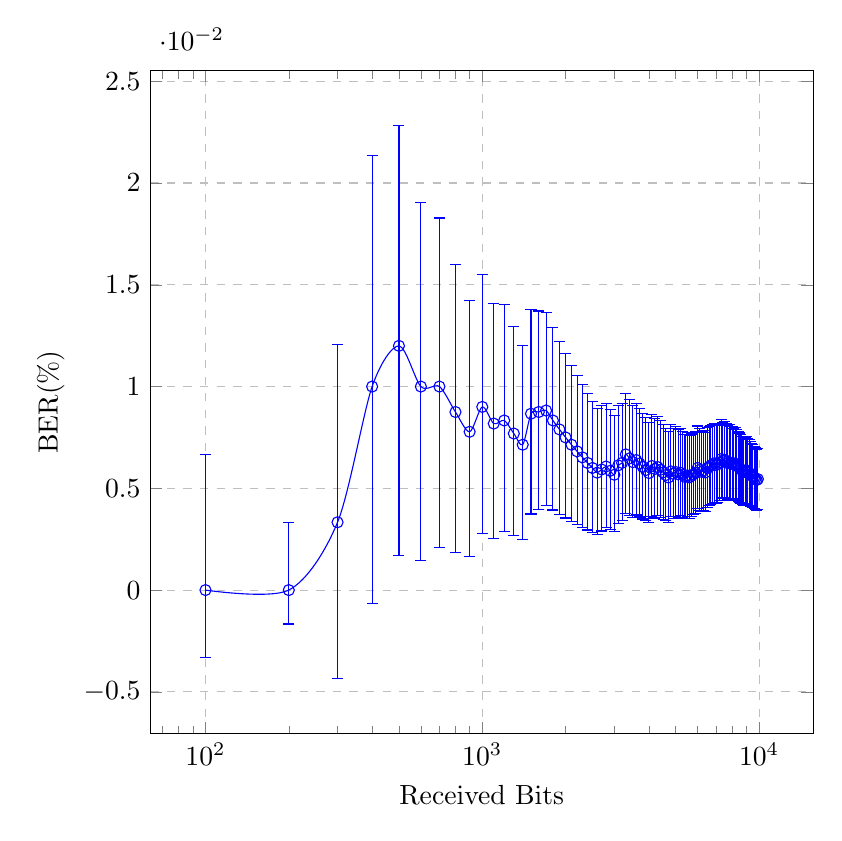
\begin{tikzpicture}
            \begin{axis}[
                height=10cm,
                width=10cm,
                xlabel=Received Bits,
                ylabel=BER(\%),
                xmode=log,
                ymajorgrids=true,
                xmajorgrids=true,
                grid style=dashed,
            ]
            \addplot[
                samples y=0,
                smooth,
                mark=o,
                blue,
                error bars/.cd, y dir=both, y explicit,
            ] plot coordinates {
                (100.0,0.0) +=(0,0.00666667) -=(0,0.00333333)
                (200.0,0.0) +=(0,0.00333333) -=(0,0.00166667)
                (300.0,0.00333333) +=(0,0.00871237) -=(0,0.00766558)
                (400.0,0.01) +=(0,0.011345) -=(0,0.010656389)
                (500.0,0.012) +=(0,0.0108079) -=(0,0.01028017)
                (600.0,0.01) +=(0,0.0090243) -=(0,0.00856521)
                (700.0,0.01) +=(0,0.0082819) -=(0,0.00788837)
                (800.0,0.00875) +=(0,0.0072552) -=(0,0.00690187)
                (900.0,0.00777778) +=(0,0.00645502) -=(0,0.00613469)
                (1000.0,0.009) +=(0,0.006494) -=(0,0.00621275)
                (1100.0,0.00818182) +=(0,0.00590798) -=(0,0.005648)
                (1200.0,0.00833333) +=(0,0.00567887) -=(0,0.00544127)
                (1300.0,0.00769231) +=(0,0.00524499) -=(0,0.00502282)
                (1400.0,0.00714286) +=(0,0.00487264) -=(0,0.00466413)
                (1500.0,0.00866667) +=(0,0.00511843) -=(0,0.00492966)
                (1600.0,0.00875) +=(0,0.0049642) -=(0,0.00478751)
                (1700.0,0.00882353) +=(0,0.00482267) -=(0,0.0046566)
                (1800.0,0.00833333) +=(0,0.00455657) -=(0,0.00439814)
                (1900.0,0.00789474) +=(0,0.00431826) -=(0,0.00416688)
                (2000.0,0.0075) +=(0,0.0041037) -=(0,0.00395871)
                (2100.0,0.00714286) +=(0,0.00390944) -=(0,0.00377036)
                (2200.0,0.00681818) +=(0,0.00373272) -=(0,0.00359911)
                (2300.0,0.00652174) +=(0,0.00357126) -=(0,0.00344275)
                (2400.0,0.00625) +=(0,0.00342322) -=(0,0.0032994)
                (2500.0,0.006) +=(0,0.00328696) -=(0,0.00316752)
                (2600.0,0.00576923) +=(0,0.00316113) -=(0,0.00304577)
                (2700.0,0.00592593) +=(0,0.00313559) -=(0,0.00302485)
                (2800.0,0.00607143) +=(0,0.00310916) -=(0,0.00300267)
                (2900.0,0.00586207) +=(0,0.00300245) -=(0,0.00289921)
                (3000.0,0.00566667) +=(0,0.00290282) -=(0,0.00280265)
                (3100.0,0.00612903) +=(0,0.00295677) -=(0,0.00286069)
                (3200.0,0.00625) +=(0,0.00293324) -=(0,0.00284038)
                (3300.0,0.00666667) +=(0,0.00297264) -=(0,0.00288333)
                (3400.0,0.00647059) +=(0,0.00288564) -=(0,0.00279862)
                (3500.0,0.00628571) +=(0,0.0028036) -=(0,0.00271875)
                (3600.0,0.00638889) +=(0,0.00278271) -=(0,0.00270039)
                (3700.0,0.00621622) +=(0,0.00270785) -=(0,0.0026275)
                (3800.0,0.00605263) +=(0,0.00263693) -=(0,0.00255842)
                (3900.0,0.00589744) +=(0,0.00256961) -=(0,0.0024929)
                (4000.0,0.00575) +=(0,0.00250565) -=(0,0.00243064)
                (4100.0,0.00609756) +=(0,0.0025412) -=(0,0.00246851)
                (4200.0,0.00595238) +=(0,0.00248096) -=(0,0.0024098)
                (4300.0,0.00604651) +=(0,0.00246809) -=(0,0.00239871)
                (4400.0,0.00590909) +=(0,0.00241225) -=(0,0.00234426)
                (4500.0,0.00577778) +=(0,0.00235887) -=(0,0.00229223)
                (4600.0,0.00565217) +=(0,0.00230781) -=(0,0.00224245)
                (4700.0,0.00553191) +=(0,0.00225891) -=(0,0.00219479)
                (4800.0,0.00583333) +=(0,0.00228972) -=(0,0.0022273)
                (4900.0,0.00571429) +=(0,0.00224318) -=(0,0.00218191)
                (5000.0,0.0058) +=(0,0.00223479) -=(0,0.00217484)
                (5100.0,0.00568627) +=(0,0.00219116) -=(0,0.00213224)
                (5200.0,0.00576923) +=(0,0.00218349) -=(0,0.0021258)
                (5300.0,0.00566038) +=(0,0.00214245) -=(0,0.00208575)
                (5400.0,0.00555556) +=(0,0.00210294) -=(0,0.00204717)
                (5500.0,0.00563636) +=(0,0.00209676) -=(0,0.00204208)
                (5600.0,0.00553571) +=(0,0.00205947) -=(0,0.00200566)
                (5700.0,0.00561404) +=(0,0.00205376) -=(0,0.002001)
                (5800.0,0.00568966) +=(0,0.0020478) -=(0,0.00199602)
                (5900.0,0.00576271) +=(0,0.00204161) -=(0,0.00199076)
                (6000.0,0.006) +=(0,0.00206229) -=(0,0.00201253)
                (6100.0,0.00590164) +=(0,0.00202863) -=(0,0.00197958)
                (6200.0,0.00580645) +=(0,0.00199604) -=(0,0.0019477)
                (6300.0,0.00587302) +=(0,0.00198993) -=(0,0.00194243)
                (6400.0,0.00578125) +=(0,0.00195897) -=(0,0.00191212)
                (6500.0,0.006) +=(0,0.00197731) -=(0,0.00193137)
                (6600.0,0.00606061) +=(0,0.00197082) -=(0,0.00192563)
                (6700.0,0.0061194) +=(0,0.00196424) -=(0,0.00191977)
                (6800.0,0.00617647) +=(0,0.00195758) -=(0,0.00191381)
                (6900.0,0.00623188) +=(0,0.00195085) -=(0,0.00190776)
                (7000.0,0.00614286) +=(0,0.0019231) -=(0,0.00188056)
                (7100.0,0.00619718) +=(0,0.00191681) -=(0,0.00187491)
                (7200.0,0.00625) +=(0,0.00191045) -=(0,0.00186918)
                (7300.0,0.00643836) +=(0,0.0019235) -=(0,0.00188295)
                (7400.0,0.00635135) +=(0,0.00189762) -=(0,0.00185754)
                (7500.0,0.0064) +=(0,0.00189115) -=(0,0.00185165)
                (7600.0,0.00631579) +=(0,0.00186638) -=(0,0.00182733)
                (7700.0,0.00623377) +=(0,0.00184224) -=(0,0.00180364)
                (7800.0,0.00628205) +=(0,0.00183655) -=(0,0.00179847)
                (7900.0,0.00620253) +=(0,0.0018134) -=(0,0.00177575)
                (8000.0,0.00625) +=(0,0.00180803) -=(0,0.00177089)
                (8100.0,0.00617284) +=(0,0.0017858) -=(0,0.00174906)
                (8200.0,0.00621951) +=(0,0.00178074) -=(0,0.00174447)
                (8300.0,0.00614458) +=(0,0.00175937) -=(0,0.00172349)
                (8400.0,0.00607143) +=(0,0.00173851) -=(0,0.00170301)
                (8500.0,0.006) +=(0,0.00171814) -=(0,0.00168301)
                (8600.0,0.00593023) +=(0,0.00169824) -=(0,0.00166347)
                (8700.0,0.00586207) +=(0,0.0016788) -=(0,0.00164439)
                (8800.0,0.00579545) +=(0,0.0016598) -=(0,0.00162573)
                (8900.0,0.0058427) +=(0,0.00165639) -=(0,0.00162274)
                (9000.0,0.00588889) +=(0,0.00165292) -=(0,0.00161967)
                (9100.0,0.00582418) +=(0,0.00163483) -=(0,0.00160191)
                (9200.0,0.00576087) +=(0,0.00161713) -=(0,0.00158452)
                (9300.0,0.00569892) +=(0,0.00159981) -=(0,0.00156751)
                (9400.0,0.0056383) +=(0,0.00158285) -=(0,0.00155087)
                (9500.0,0.00557895) +=(0,0.00156625) -=(0,0.00153457)
                (9600.0,0.00552083) +=(0,0.00155) -=(0,0.0015186)
                (9700.0,0.00546392) +=(0,0.00153408) -=(0,0.00150298)
                (9800.0,0.00540816) +=(0,0.00151849) -=(0,0.00148766)
                (9900.0,0.00545455) +=(0,0.00151659) -=(0,0.00148612)

            };
            \end{axis}
        \end{tikzpicture}
        \end{center}
        It is interesting to observe how the confidence bounds shrink, and that the BER value is within the previous values of these bounds (in at least $(1-\alpha)\%$ of the cases).


\end{itemize}






\subsection*{Functional and Theoretical Description}

This block accepts two binary strings and outputs a binary string. For each pair of input bits, it outputs a '1' if the two coincide and '0' if not.
\\
The $\widehat{\text{BER}}$ is thus obtained by counting both the total number received bits, $N_{bits}$, and the number of coincidences, $K$, and calculating their relative ratio:
\begin{equation}
\widehat{\text{BER}}=1-\frac{K}{N_{bits}}.
\end{equation}
\\
The confidence interval of the $\widehat{\text{BER}}$ value is also calculated. To easily obtain the upper and lower bounds, $\text{BER}_\text{UB}$ and $\text{BER}_\text{LB}$ respectively, an approximation of the Clopper-Pearson confidence interval~\cite{Almeida16} is used, which holds valid for $N_{bits}>40$:
\begin{align}
\text{BER}_\text{UB}&=\widehat{\text{BER}}+\frac{z_{\alpha/2}}{\sqrt{N_{bits}}}\sqrt{\widehat{\text{BER}}(1-\widehat{\text{BER}})}+\frac{1}{3N_{bits}}\left[2\left(\frac{1}{2}-\widehat{\text{BER}}\right)z_{\alpha/2}^2+2-\widehat{\text{BER}}\right]\\
\text{BER}_\text{LB}&=\widehat{\text{BER}}-\frac{z_{\alpha/2}}{\sqrt{N_{bits}}}\sqrt{\widehat{\text{BER}}(1-\widehat{\text{BER}})}+\frac{1}{3N_{bits}}\left[2\left(\frac{1}{2}-\widehat{\text{BER}}\right)z_{\alpha/2}^2-1-\widehat{\text{BER}}\right]
\end{align}
where $z_{\alpha/2}$ is the $100\left(1-\frac{\alpha}{2}\right)$th percentile of a standard normal distribution and this is where the value of the \textit{alpha} parameter influences the result.
\\
Upon finishing running, this block outputs to the \textit{signals} directory a file named \textit{BER.txt} with a report of the estimated $\widehat{\text{BER}}$, the estimated confidence bounds for a given confidence level ($1-\alpha$) and the total number of received bits.
\\
The file format is the following:
\begin{adjustwidth}{1.5cm}{}
\begin{verbatim}
BER= 4.34783e-05
Upper and lower confidence bounds for 95% confidence level
Upper Bound= 9.33303e-05
Lower Bound= 1.47979e-05
Number of received bits =92000
\end{verbatim}
\end{adjustwidth}
Another functionality of the BER block is that it allows for mid-reports to be generated. A mid-report has exactly the same structure of the final report showed above, but it's generated for every \textit{m} pairs of input bits. These files are saved in the same directory of the running solution and they're saved on files named \textit{midreport\#.txt}, where the '\#' stands for the number of the respective mid-report and is in the interval [$1;\frac{N_{bits}}{m}$].
\\
The number of bits between reports is the parameter \textit{m}, customizable, and if it is set to '0' then the block will only output the final report.

\subsection*{Open Issues}
\begin{itemize}
  \item[--] The output value for the Lower bound is negative when the BER is null, and in these cases it should be set to '0'. This error is hidden in the \textit{BER.txt} file, because when the Lower Bound value is lower than the \textit{lMinorant} parameter, an \textit{if} statement sets it to the value of \textit{lMinorant}. This correction can however lead to errors in the cases that the \textit{lMinorant} is smaller than the actual BER we're attempting to measure.

  \item[--] Mid-reports are not formatted exactly like the BER output file. And they are stored in the current directory, instead of being saved in the same directory as the \textit{BER.txt} file, which would probably be more desirable.
\end{itemize}

\subsection*{Future Improvements}
\begin{itemize}
    \item[--] fixing the Lower Bound issue mentioned above;
    \item[--] the printing of all the mid-reports could be done in the same file, for ease of BER convergence analysis;
    \item[--] the method \textit{getLowestMinorant()} should have a \textit{const} return;
    \item[--] there could be only one private method for printing an output file, thus avoiding having two times the same code repeated for the mid-report printing and for the BER final report printing;
    \item[--] exactness required for the convergence of the z-score should also be a parameter, for it may be desirable to have a different value of exactness.
\end{itemize}

% bibliographic references for the section ----------------------------
\printbibliography[heading=subbibliography]
\end{refsection}
\addcontentsline{toc}{subsection}{Bibliography}
\cleardoublepage
% --------------------------------------------------------------------- 